\chapter{Конструкторский раздел}

В данном разделе представлены требования к ПО, описание работы алгоритмов построения и визуализации трехмерной сцены; приведена структура программного обеспечения.

\section{Требования к программному обеспечению}
Программа должна удовлетворять следующим требованиям:
\begin{itemize}
	\item характеристики генерирования ландшафта задаются пользователем через графический интерфейс;
	\item расположение источника света задается через интерфейс;
	\item размер сцены, а также поворот и масштабирование ландшафта задаются в интерфейсе.
\end{itemize}

\section{Описание работы алгоритмов}
На рисунке \ref{png:convert_to_image} представлена схема алгоритма построения 3D изображения на экране.
\begin{figure}[H]
	\centering{
		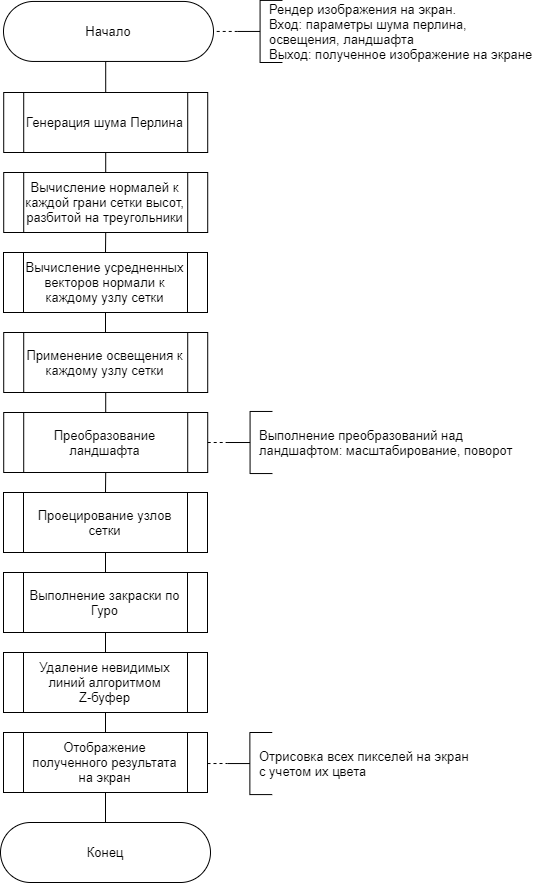
\includegraphics[scale=0.6]{../../../../../../../msys64/home/Лев/bmstu_cg_course_project/rpz/diagrams/convert_to_image}
		\caption{Схема алгоритма построения 3D изображения на экране}
		\label{png:convert_to_image}
			}
\end{figure}

\newpage
На рисунках \ref{png:perlin_1_schema}, \ref{png:perlin_2_schema}  и \ref{png:perlin_3_schema} представлены схемы алгоритма генерирования карты высот на основе шума Перлина.
\begin{figure}[H]
	\captionsetup{justification=centering}
	\centering{
		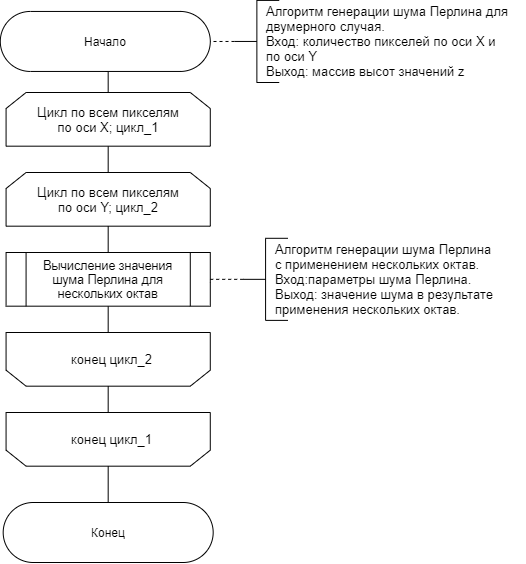
\includegraphics[scale=0.6]{../../../../../../../msys64/home/Лев/bmstu_cg_course_project/rpz/diagrams/perlin_1}
		\caption{Схема алгоритма построения шума Перлина для двумерного случая}
		\label{png:perlin_1_schema}
	}
\end{figure}

\begin{figure}[H]
	\captionsetup{justification=centering}
	\centering{
		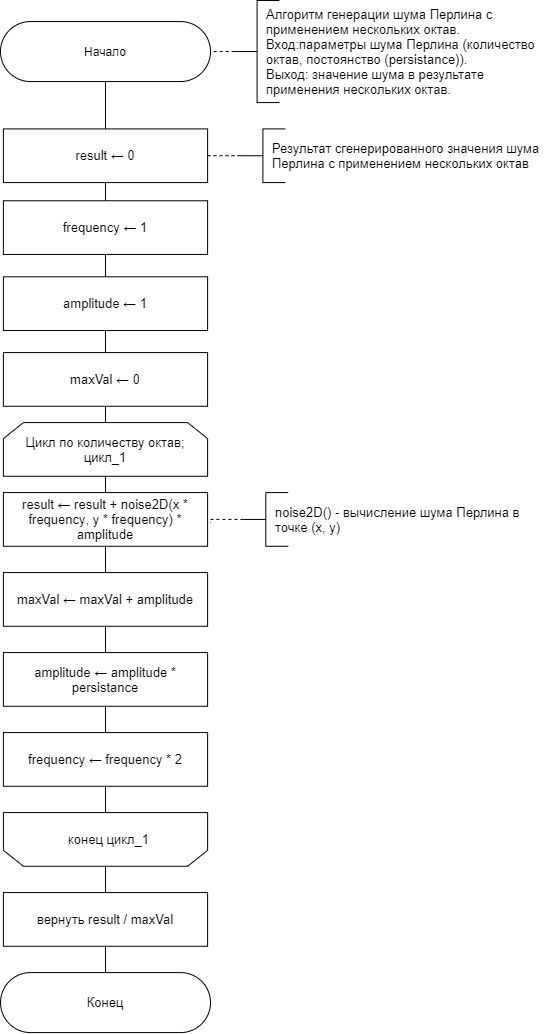
\includegraphics[scale=0.6]{../../../../../../../msys64/home/Лев/bmstu_cg_course_project/rpz/diagrams/perlin_2}
		\caption{Схема алгоритма шума Перлина в зависимости от числа октав}
		\label{png:perlin_2_schema}
	}
\end{figure}

\begin{figure}[H]
	\centering{
		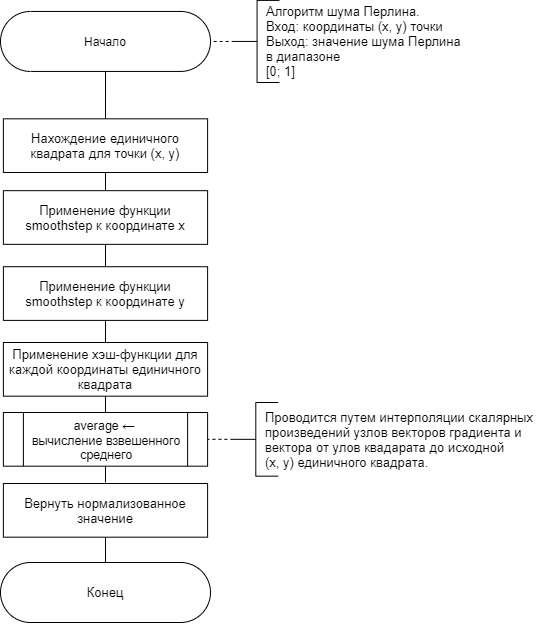
\includegraphics[scale=0.6]{../../../../../../../msys64/home/Лев/bmstu_cg_course_project/rpz/diagrams/perlin_3}
		\caption{Схема алгоритма шума Перлина}
		\label{png:perlin_3_schema}
	}
\end{figure}

\newpage
На рисунке \ref{png:guro_shading_schema} представлена схема алгоритма закраски Гуро.
\begin{figure}[H]
	\centering{
		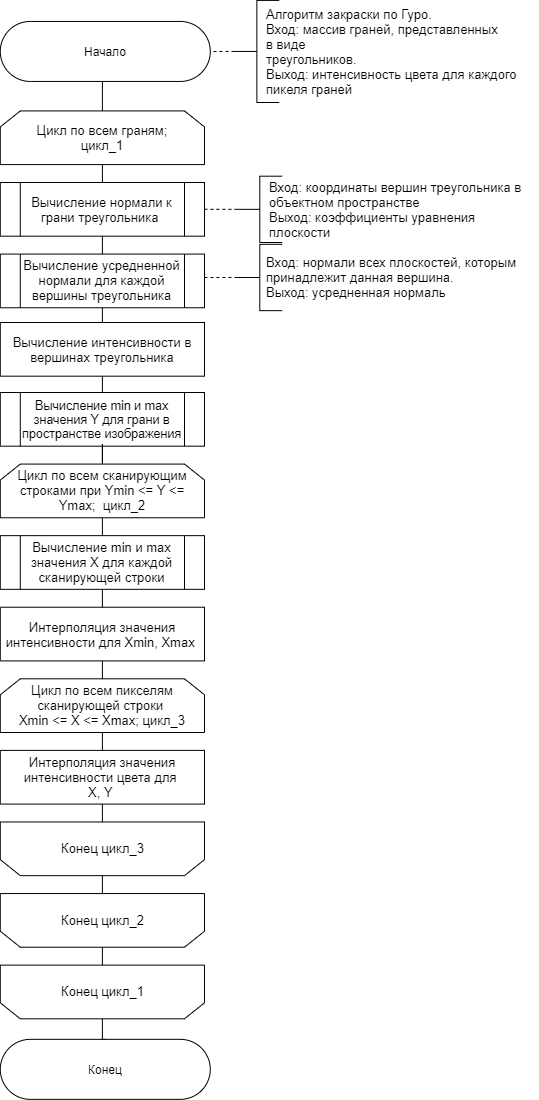
\includegraphics[scale=0.6]{../../../../../../../msys64/home/Лев/bmstu_cg_course_project/rpz/diagrams/guro_shading}
		\caption{Схема алгоритма закраски Гуро}
		\label{png:guro_shading_schema}
	}
\end{figure}

На рисунке \ref{png:zbuffer_schema} представлена схема алгоритма Z-буфер.
\begin{figure}[H]
	\centering{
		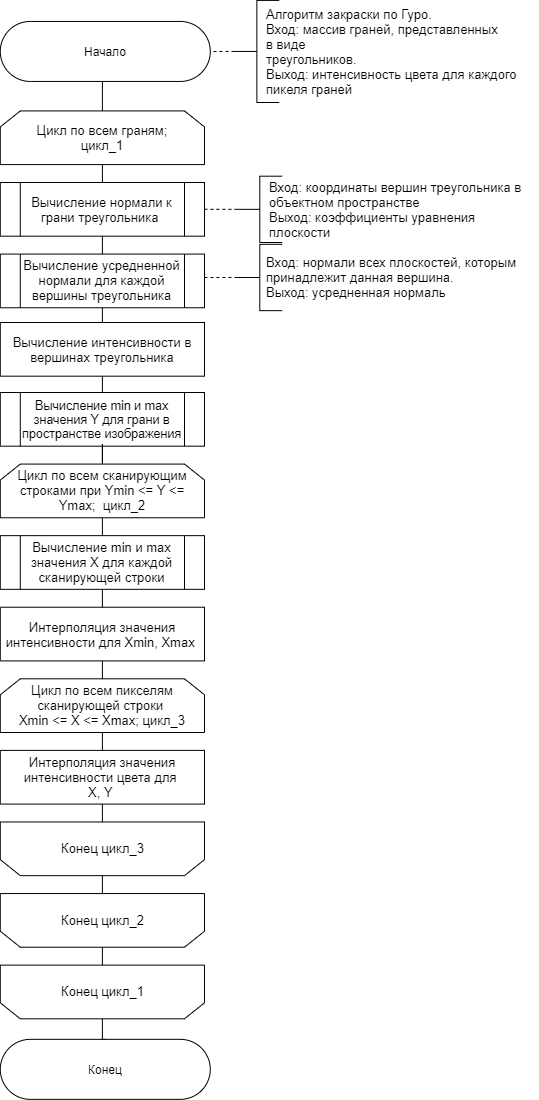
\includegraphics[scale=0.6]{../../../../../../../msys64/home/Лев/bmstu_cg_course_project/rpz/diagrams/guro_shading}
		\caption{Схема алгоритма Z-буфер}
		\label{png:zbuffer_schema}
	}
\end{figure}

На рисунках \ref{png:zbuffer_guro_schema_1} и \ref{png:zbuffer_guro_schema_2} представлены схемы алгоритма Z-буфер в сочетании с закраской Гуро.
\begin{figure}[H]
	\centering{
		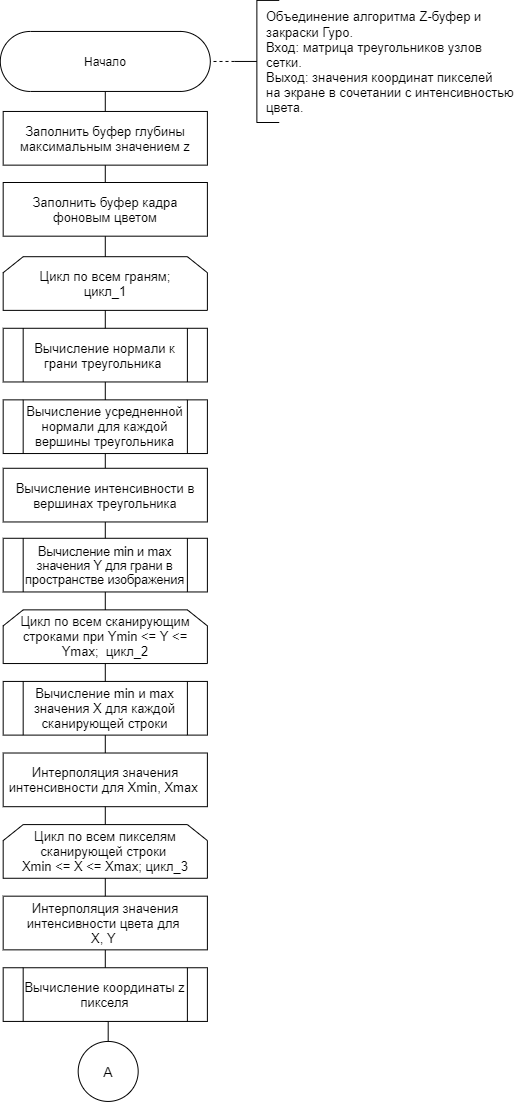
\includegraphics[scale=0.55]{../../../../../../../msys64/home/Лев/bmstu_cg_course_project/rpz/diagrams/guro_plus_zbuffer_1}
		\caption{Схема алгоритма Z-буфер в сочетании с закраской Гуро}
		\label{png:zbuffer_guro_schema_1}
	}
\end{figure}

\begin{figure}[H]
	\centering{
		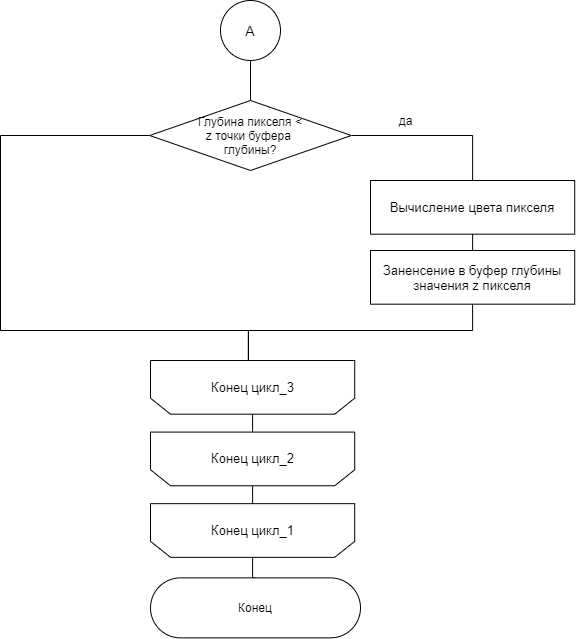
\includegraphics[scale=0.55]{../../../../../../../msys64/home/Лев/bmstu_cg_course_project/rpz/diagrams/guro_plus_zbuffer_2}
		\caption{Схема алгоритма Z-буфер в сочетании с закраской Гуро}
		\label{png:zbuffer_guro_schema_2}
	}
\end{figure}

\section{Шум Перлина}
Пусть (i,j) обозначают четыре точки на этом квадрате, где $i$ - набор нижних и верхних ограничивающих целых чисел на $x: \{|x|,|x| + 1\}$, и аналогично $j = \{|y|,|y| + 1\}$. Четыре градиента задаются через $g_{i,j} = G[P[P[i]+j]]$, где предварительно вычисленные массивы P и G содержат, соответственно, псевдослучайную перестановку и псевдослучайную единичный вектор градиента. Четыре линейные функции $g_{i,j} · (x_{i}, y_{j})$ затем билинейно интерполируются с помощью $s(x-|x|),\ s(y-|y|), где s(t) = 6t^5 - 15t^4 + 10t^3$.

\section{Структура программного обеспечения}
В качестве парадигмы было использовано объектно-ориентированное программирование. На рисунке \ref{png:diagram_class} представлена диаграмма классов ПО.
\begin{figure}[H]
	\centering{
		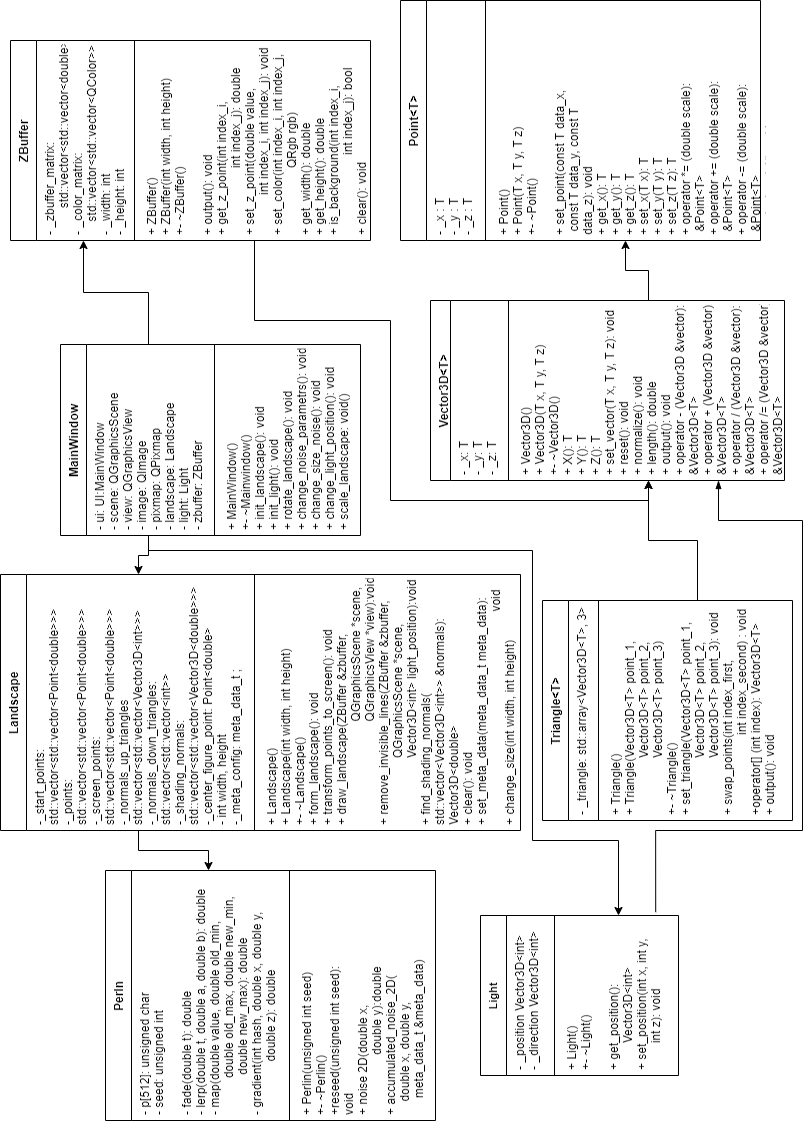
\includegraphics[scale=0.65]{../../../../../../../msys64/home/Лев/bmstu_cg_course_project/rpz/diagrams/diagram_class}
		\caption{Диаграмма классов}
		\label{png:diagram_class}
	}
\end{figure}

Были спроектированы следующие классы:
\begin{itemize}
	\item Perlin - хранит таблицу перестановок p и значение "зерна"\ seed;
	\item Light - хранит позиию точечного источника освещения и его направление до точки (x, y);
	\item Landscape - хранит объектные точки, экранные точки, нормали к треугольникам, усредненные нормали, координату центра ландшафт, линейные размеры ландшафта и параметры шума Перлина;
	\item ZBuffer - хранит информацию о буфеер кадра и буфере глубины.
\end{itemize}

\section{Описание оптимизации временных характеристик}
Из схемы алгоритмов \ref{png:guro_shading_schema} и \ref{png:zbuffer_schema} следует, что каждый раз выполняется обработка всех пикселей карты высот. В связи с этим будет целесообразней совместить алгоритм Z-буфер и закраски Гуро как на рисунках \ref{png:zbuffer_guro_schema_1} и \ref{png:zbuffer_guro_schema_2}. 

\section{Использование матричных фильтров}
Для более гибкой работы с ландшафтом стоит учесть такой параметр как «редактирование». Этот этап позволит пользователю изменять желаемые настройки при работе с ландшафтом. Например, при использовании матричного фильтра, который может использовать матрицу размером $m\times n$, элементы которой соответствуют коэффициентам увеличения высоты в отдельной области ландшафта.

\section{Использование стохастических алгоритмов}
Стохастичность означает случайность. Стохастические алгоритмы могут вносить случайный фактор в формирование положения сетки ландшафта в мировом пространстве. Например, они могут изменять исходный ландшафт при одинаковых параметрах таким образом, чтобы каждый раз выводился совершенно новый результат.

Например, можно при помощи случайности можно задавать настройки шума Перлина так, чтобы можно было выводить различные изображения на экране. Другим применением таких алгоритмов можно задавать положение ландшафта в пространстве путем переопределения его местоположения в пространстве или же вывод на экран только небольшой части ландшафта.

\section{Вывод}
Были описаны алгоритмы визуализации сцены и генерирования ландшафта предложен метод оптимизации. Было спроектировано программное обеспечение и представлены требования к ПО.